Figure~\ref{fig:curve} shows the training loss and the validation macro-F1 used to pick the checkpoint.
The selected epoch is 1, with validation macro-F1 0.458 during training.
0 train rows lost an expert sentence id to truncation at the trained length.
The 601 teaching annotations were repeated only inside the train split, up to the majority count of each criterion type and at most eight times, which produced 1190 encoded rows.

\begin{figure}[t]
\centering
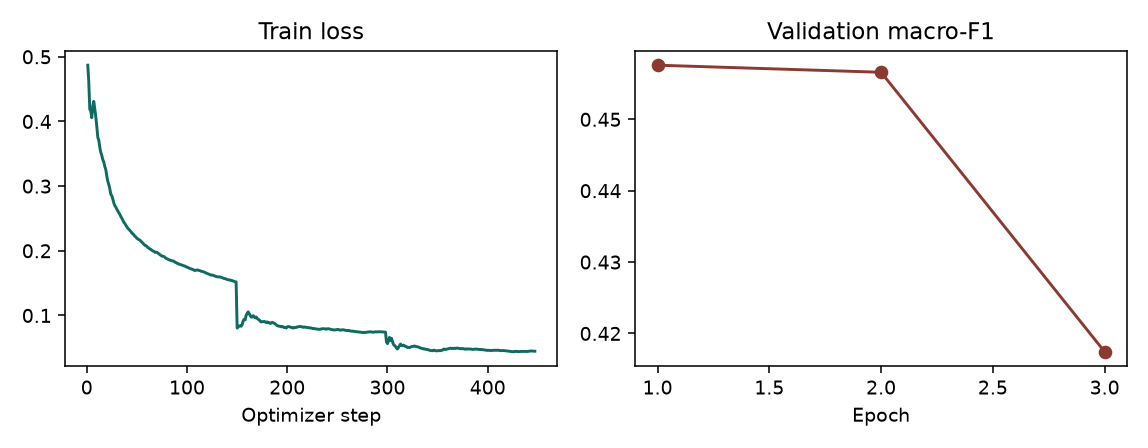
\includegraphics[width=0.95\linewidth]{../results/task1/training_curve.png}
\caption{Train loss by optimizer step and validation macro-F1 by epoch. The checkpoint with the higher validation macro-F1 is the one that is evaluated.}
\label{fig:curve}
\end{figure}

Table~\ref{tab:compare} compares the untouched base model and the adapter on the same rows and the same greedy decoder.
On validation, accuracy moves from 9.2\% to 67.5\% and macro-F1 moves from 0.108 to 0.458.
On the held-out test set, which was scored once, accuracy is 10.7\% for the base model and 67.5\% for the adapter.
Test macro-F1 is 0.150 and 0.492.
Example-level evidence F1 on the test set is 0.214 and 0.724.

\begin{table}[t]
\centering
\caption{Base model and adapter. Decoding is greedy. The test split was scored once.}
\label{tab:compare}
\begin{tabular}{lcccc}
\toprule
Split & Model & Accuracy & Macro-F1 & Evidence F1 \\
\midrule
Validation & Base & 9.2\% & 0.108 & 0.164 \\
Validation & Adapter & 67.5\% & 0.458 & 0.646 \\
Test & Base & 10.7\% & 0.150 & 0.214 \\
Test & Adapter & 67.5\% & 0.492 & 0.724 \\
\bottomrule
\end{tabular}
\end{table}

Table~\ref{tab:perclass} is the adapter's per-class precision, recall, and F1 on the test set.
Rare labels stay rare: a high accuracy can still hide a weak F1 on ``excluded'' or ``not included''.
Figure~\ref{fig:cm} is the adapter's test confusion matrix.
The inclusion and exclusion matrices are saved beside it and are not a collapsed yes/no task.

\begin{table}[t]
\centering
\caption{Adapter, test set, per-class scores. Support is the number of expert labels.}
\label{tab:perclass}
\begin{tabular}{lcccc}
\toprule
Label & Support & Precision & Recall & F1 \\
\midrule
included & 27 & 0.880 & 0.815 & 0.846 \\
not included & 7 & 0.238 & 0.714 & 0.357 \\
excluded & 0 & 0.000 & 0.000 & 0.000 \\
not excluded & 91 & 0.730 & 0.923 & 0.816 \\
not enough information & 66 & 0.769 & 0.303 & 0.435 \\
not applicable & 15 & 0.471 & 0.533 & 0.500 \\
\bottomrule
\end{tabular}
\end{table}

\begin{figure}[t]
\centering
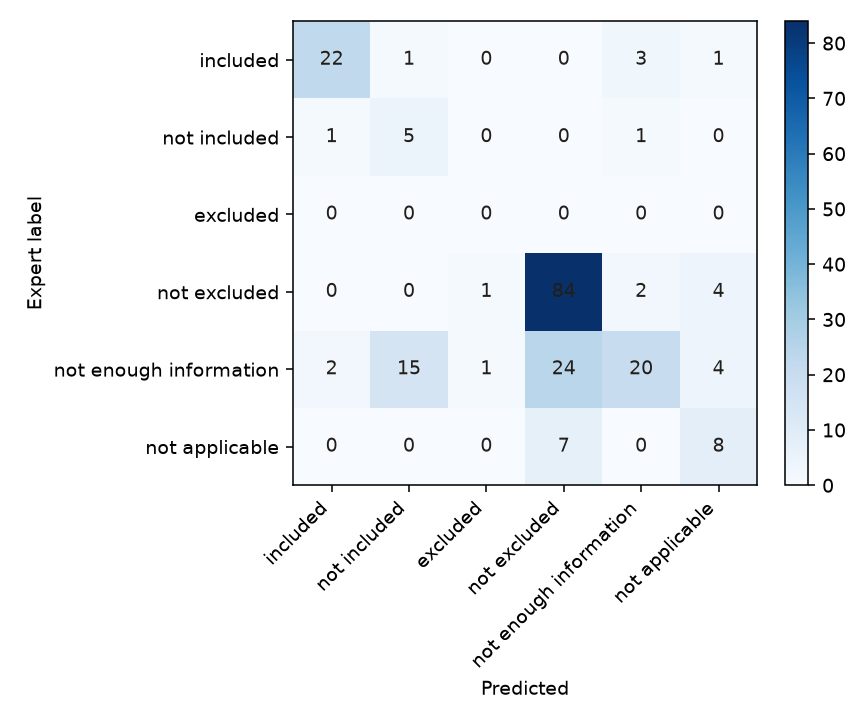
\includegraphics[width=0.72\linewidth]{../results/task2/confusion_test_adapter_overall.png}
\caption{Confusion matrix for the adapter on the test set. Rows are expert labels and columns are predictions. Unparsed outputs are their own column.}
\label{fig:cm}
\end{figure}

Table~\ref{tab:evidence} applies the empty-set rule to the adapter on the test set.
Both-empty counts as a match. A citation where the expert cited nothing scores zero, and so does a missing citation where the expert cited something.

\begin{table}[t]
\centering
\caption{Adapter evidence scores on the test set. Macro is the mean of the example scores. Micro pools sentence occurrences.}
\label{tab:evidence}
\resizebox{\columnwidth}{!}{%
\begin{tabular}{lcccccc}
\toprule
Slice & P & R & F1 & Micro P & Micro R & Micro F1 \\
\midrule
Overall & 0.719 & 0.743 & 0.724 & 0.380 & 0.660 & 0.482 \\
Inclusion & 0.567 & 0.613 & 0.574 & 0.407 & 0.742 & 0.526 \\
Exclusion & 0.805 & 0.818 & 0.809 & 0.320 & 0.500 & 0.390 \\
\bottomrule
\end{tabular}}
\end{table}

The base model left 0 test outputs unparsed.
The adapter left 0 unparsed and cited an id outside the note on 0 rows.
Table~\ref{tab:errors} lists the reviewed failures. Each row in the accompanying \texttt{errors.md} stores the criterion, the expert label, the prediction, the quoted sentences, and why it failed.

\begin{table}[t]
\centering
\caption{Reviewed test failures for the adapter. The full quotations are in \texttt{results/task2/errors.md}.}
\label{tab:errors}
\resizebox{\columnwidth}{!}{%
\begin{tabular}{llccc}
\toprule
Category & Id & Type & Expert & Predicted \\
\midrule
wrong\ label & 164 & inclusion & not included & included \\
missing\ information & 169 & exclusion & not enough information & not excluded \\
missed\ gold\ sentence & 185 & inclusion & included & not enough information \\
empty\ gold\ but\ model\ cited & 161 & inclusion & not included & not included \\
not\ applicable\ confusion & 683 & exclusion & not applicable & not excluded \\
additional\ mismatch & 162 & inclusion & not included & not included \\
additional\ mismatch & 163 & inclusion & not included & not included \\
additional\ mismatch & 166 & exclusion & not excluded & not excluded \\
truncation\ would\ drop\ gold & 160 & inclusion & included & included \\
\bottomrule
\end{tabular}}
\end{table}

Table~\ref{tab:kv} checks the hand-written cache against the uncached loop on the adapter model.
Tokens match on 2 of 3 graded lengths. At 32/16 the first disagreement is index 42: the cache emits token 19 and the uncached loop emits token 20. A fresh one-step cache on that shared prefix agrees with the full forward. The top logits differ by one bf16 unit, so the long-running cache breaks a tie. The position ids and the mask are the same on both paths.
Prefill is timed separately from the later tokens.
The first new token is produced by the prefill, so the decode rate does not include it in the same way the speculative rate does.
The uncached loop resends the whole prefix, which is why its decode time grows with the prompt length.

\begin{table*}[t]
\centering
\caption{Cached and uncached greedy decoding. EOS is disabled. Times are seconds after one warmup. Memory is peak megabytes.}
\label{tab:kv}
\begin{tabular}{lcccccccc}
\toprule
Length & Equal & Prefill & Dec. cache & Dec. plain & Tok/s c. & Tok/s p. & MB c. & MB p. \\
\midrule
32/16 & false & 0.053 & 0.535 & 0.949 & 29.9 & 16.9 & 3161 & 3161 \\
128/32 & true & 0.098 & 1.033 & 4.527 & 31.0 & 7.1 & 3170 & 4194 \\
512/64 & true & 0.289 & 2.174 & 23.769 & 29.6 & 2.7 & 4218 & 4186 \\
\bottomrule
\end{tabular}
\end{table*}

Table~\ref{tab:attn} compares reference attention with tiled online softmax in fp32.
The largest absolute error in these cases is 5.96e-07.
The tiled loop is slower. That is the expected result for a Python block loop against a single matrix softmax, and it is not a fused kernel.

\begin{table}[t]
\centering
\caption{Reference and tiled attention. Shapes are batch, heads, sequence, and head size. Times are seconds.}
\label{tab:attn}
\resizebox{\columnwidth}{!}{%
\begin{tabular}{lcccccc}
\toprule
Shape & Block & Causal & Max abs & Mean abs & Ref. & Tiled \\
\midrule
1,1,8,16 & 4 & true & 1.19e-07 & 2.37e-08 & 0.00004 & 0.00006 \\
2,4,17,32 & 8 & true & 5.96e-07 & 4.45e-08 & 0.00005 & 0.00013 \\
1,2,64,64 & 16 & true & 3.58e-07 & 2.73e-08 & 0.00005 & 0.00019 \\
1,2,64,64 & 16 & false & 4.77e-07 & 2.57e-08 & 0.00003 & 0.00017 \\
1,4,128,64 & 32 & true & 4.77e-07 & 2.71e-08 & 0.00014 & 0.00042 \\
\bottomrule
\end{tabular}}
\end{table}

Table~\ref{tab:spec} is greedy speculative decoding with lookahead 4.
The draft is the 0.5\,B base model and the target is the adapter 1.5\,B model.
3 of 4 prompts matched the target's ordinary greedy tokens.
On the prompt that differs, the full-forward top two logits also differ by one bf16 unit, and the speculative token is that forward's argmax.
Acceptance rate is the fraction of drafted tokens that were kept.
A speedup below 1 is a slowdown. The token match is the correctness result.

\begin{table}[t]
\centering
\caption{Speculative decoding against target greedy decoding. 32 new tokens, lookahead 4.}
\label{tab:spec}
\resizebox{\columnwidth}{!}{%
\begin{tabular}{lcccccc}
\toprule
Prompt & Equal & Accept & Greedy tok/s & Spec. tok/s & Speedup & Peak MB \\
\midrule
1 & true & 0.622 & 20.8 & 13.8 & 0.663 & 4193 \\
2 & false & 0.447 & 16.5 & 9.7 & 0.589 & 4201 \\
3 & true & 0.667 & 24.8 & 20.4 & 0.823 & 4193 \\
4 & true & 0.622 & 23.6 & 17.0 & 0.721 & 4193 \\
\bottomrule
\end{tabular}}
\end{table}
